
\begin{Slide}{Different aspects of requirements to model }

\begin{minipage}[t]{0.6\textwidth}
\begin{itemize}
\item Functional aspects:
\begin{itemize}
\item Data aspects:
\begin{itemize}
\item What is stored and processed by the system?
\item What is the format of input and output data?

\end{itemize}
\item Business Logic aspects: 
\begin{itemize}
\item How should the system behave in different usage contexts?
\item What output should be produced, given input and state?  
\end{itemize}
\end{itemize}
\end{itemize}
\end{minipage}%
\begin{minipage}[t]{0.4\textwidth}
\vspace{0.0em}\hfill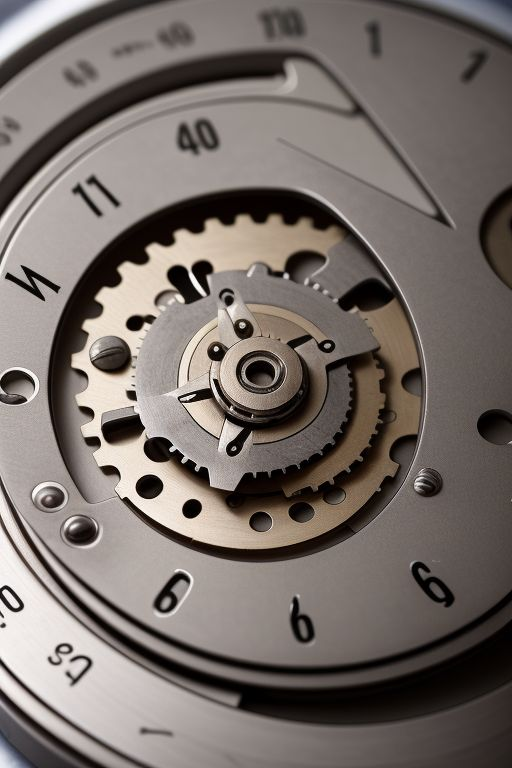
\includegraphics[width=0.82\textwidth]{../img/cog1}
\end{minipage}%

\begin{itemize}
\item Quality aspects: 
\begin{itemize}
\item What is a 'good' function from stakeholders' viewpoints?
\item More on quality modeling in Part III.

\end{itemize}
\end{itemize}
\end{Slide}